\documentclass{article}

\usepackage{../preamble}
\standalonetrue

\pagestyle{fancy}
\fancyhf{}
\rhead{Section \thesection}
\lhead{PHYS 304 Lecture 19}
\rfoot{Page \thepage}


\title{PHYS 304 Lecture 19}
\author{Ashtan Mistal}
\date{!!!}

\begin{document}

\ifstandalone
\maketitle
\fi

\graphicspath{{./Lecture19/}}

\section{Review of key points from last lecture}

Two distinct uncertainty relations, one in terms of the variances of two observables, the other in terms of the variance of energy and a time over which some other observable might noticeably change.  Both are specific to a particular state of the system, and both specify inequalities that must be satisfied.

Implications are subtle, especially when considering stationary states, where variances can be zero, or arbitrarily close to zero.

Useful to systematically make the transition from 1D to 3D in steps: i) total energy for classical treatment of single electron in 3D, expressed in terms of position and momentum \textbf{vectors}, ii) convert to a basis-agnostic Hamiltonian operator just by “adding hats” to the position and momentum operators (both of them!!), iii) then render in the QM position basis, first using cartesian coordinate system to express the vector components. 

Other than this generalized 3D version of the time-independent SE, the rest of the generic steps in finding a general solution for the time-dependent wavefunction in position space are unchanged from 1D. Recall though that the inner product of two functions must be generalized to a 3D integral over all 3D space (a volume).  Related, the probability for finding a particle in some volume $dx dy dz \equiv d \vec{r}$ located at $x_0, y_0, z_0 \equiv \vec{r_0}$ is $|\Psi(\vec{r}_0)|^2$. 

Adding more than 1D brings rotational motion into play, which in the QM context, means there are a lot more “interesting” observable operators to define and work with (e.g. angular momentum)

1D:

$$\int_{- \infty}^\infty \Psi^*(x) \Psi(x) dx \rightarrow |\Psi(x)|^2 dx$$

$\propto$ probability of finding particle within $\Delta x$ of $x$. 

3D:

$$\int \int \int \Psi^*(\vec{r}) dr \Psi(\vec{r}) d \vec{r} \rightarrow |\Psi(\vec{r})|^2 d \vec{r}$$

where $d \vec{r} = dx dy dz$ and $|\Psi(\vec{r})|^2 d \vec{r} \propto$ probability of finding particle within $\Delta \vec r$ of $\vec r$. 


\section{Infinite cubic square well potential, continued}

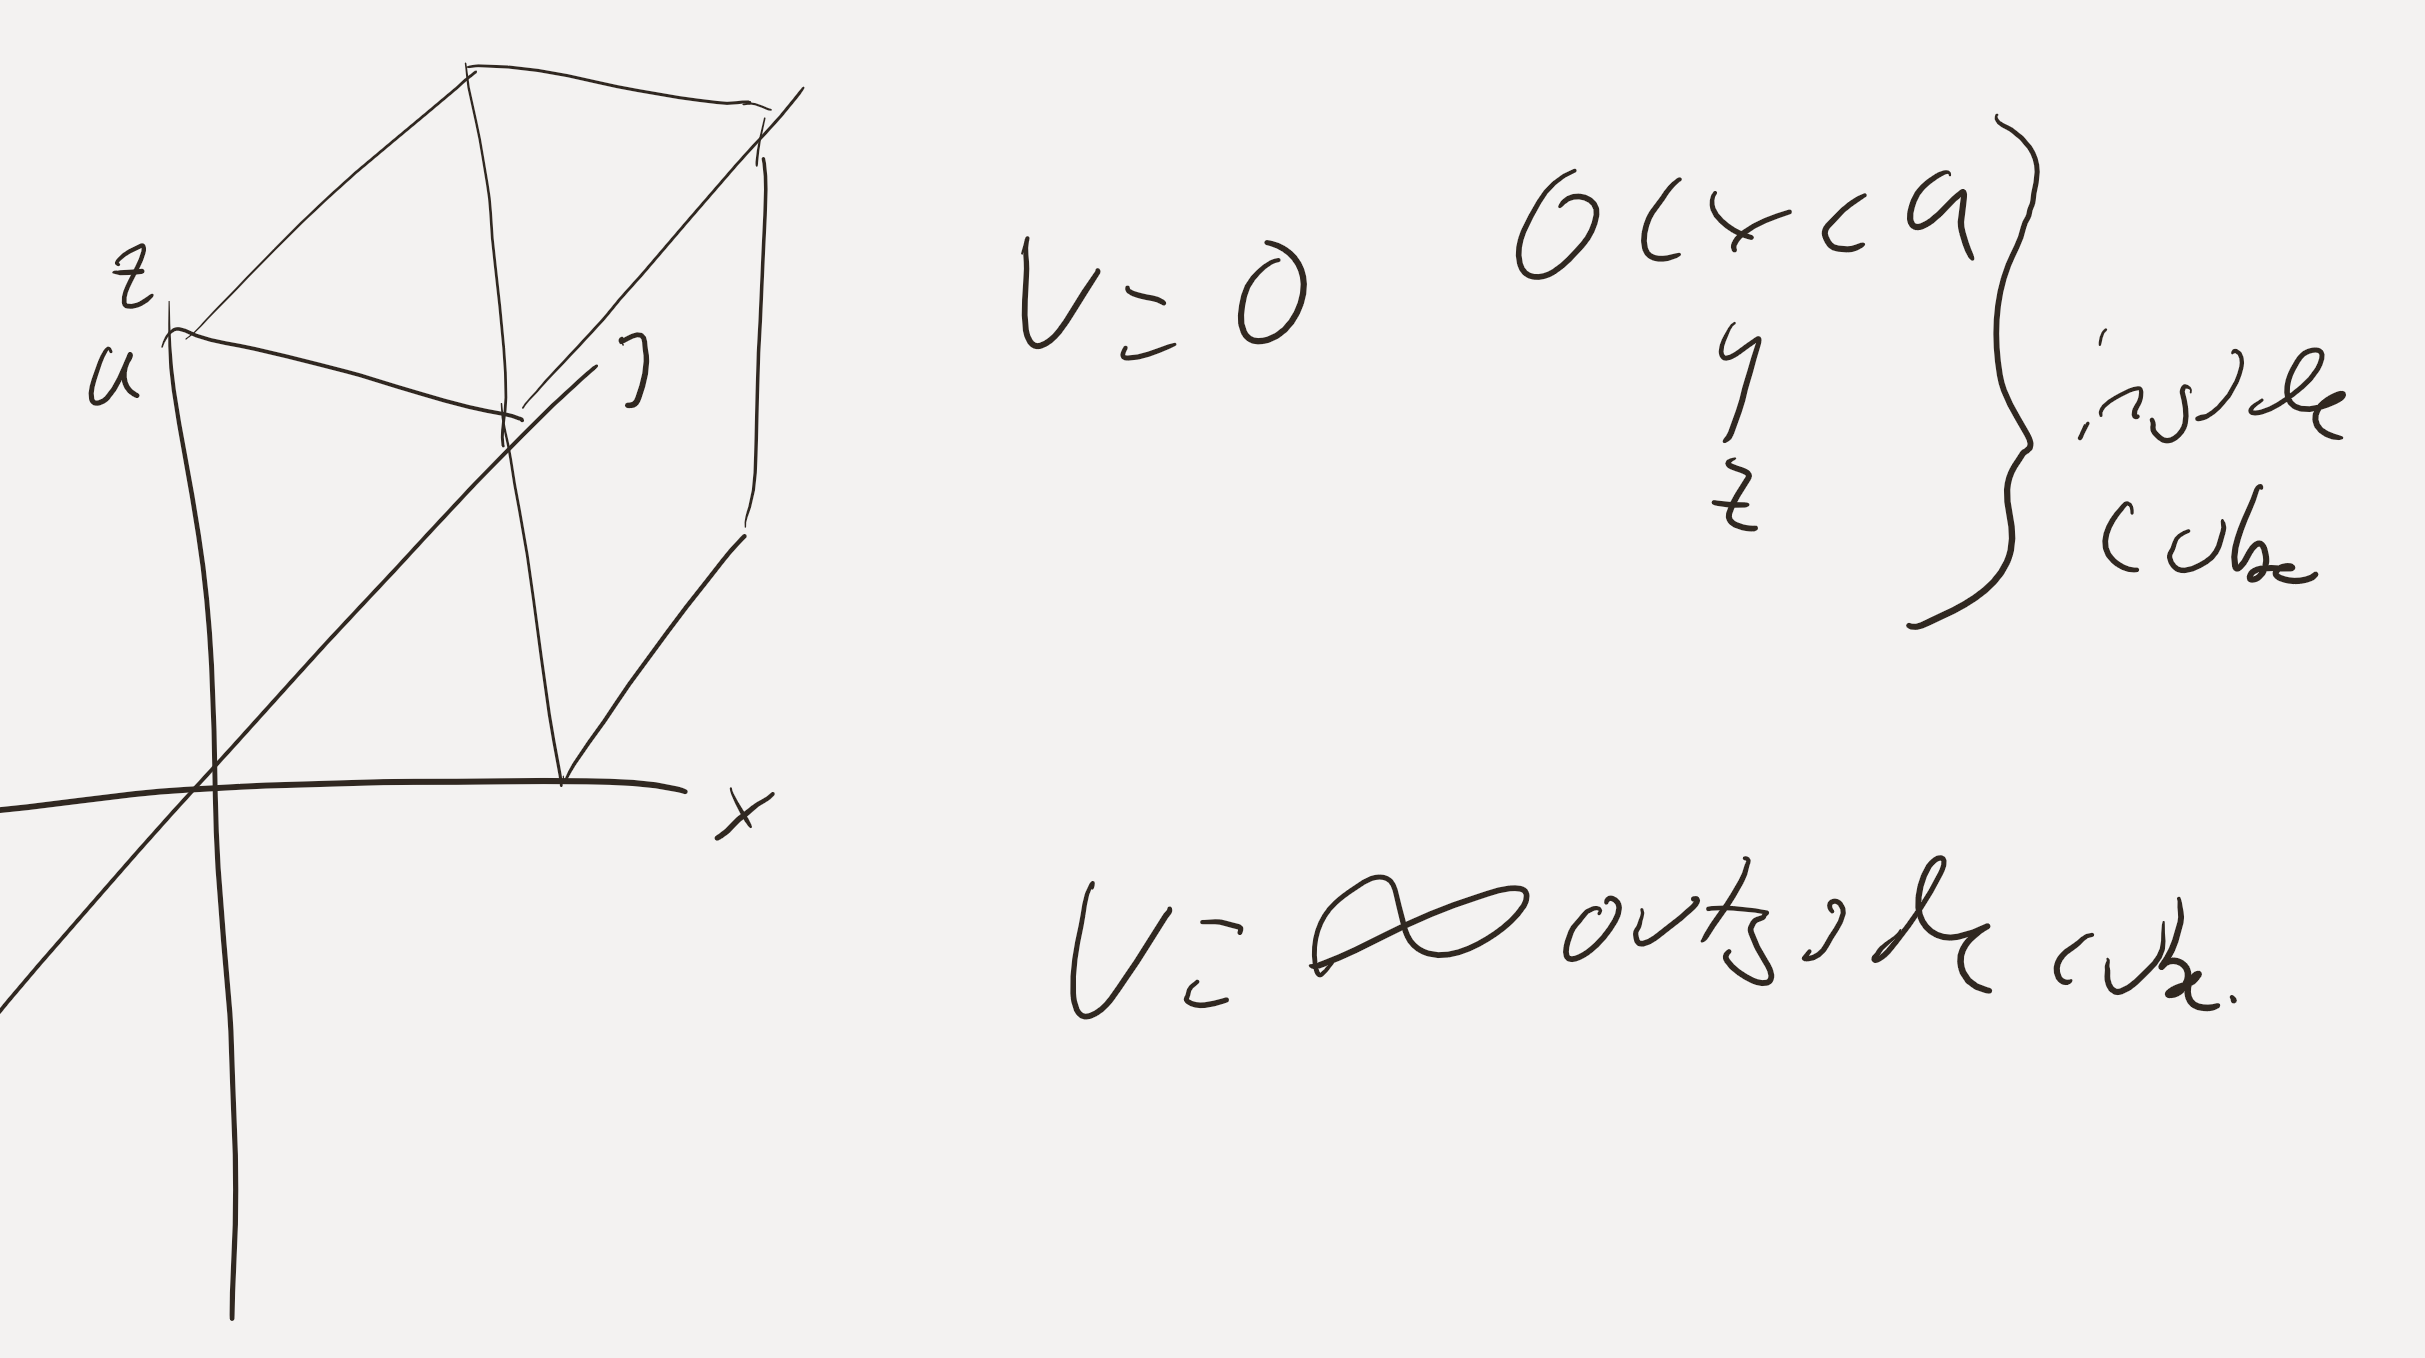
\includegraphics[width = 0.6 \textwidth]{Lecture18/3.png}

$n_1 - 1$ is the number of nodes of WF in $\text{i}^\text{th}$ direction. 

Also, $n$ related to $\braket{\hat{p}}$ in a given eigen state $\sin \left( \frac{n \pi x}{a} \right) \propto e^{ikx} - e^{-ikx}$

The solution of the 3D time independent SE for a potential that is infinite everywhere except inside a cube with one corner at the origin, $(0,0,0),$ and one at $(a,a,a).$

$\psi_{n_x, n_y, n_z} (x,y,z) = \left( \frac{2}{a} \right)^{\frac{3}{2}} \sin \left( \frac{n_x \pi x}{a} \right) \left( \frac{n_y \pi y}{a} \right) \left( \frac{n_z \pi z}{a} \right)$

$\frac{\hbar k}{m} = p$ if in a free particle state; $\propto e^{ikx}$

$\Rightarrow$ Energy (kinetic) related to number of nodes / length in square well. 

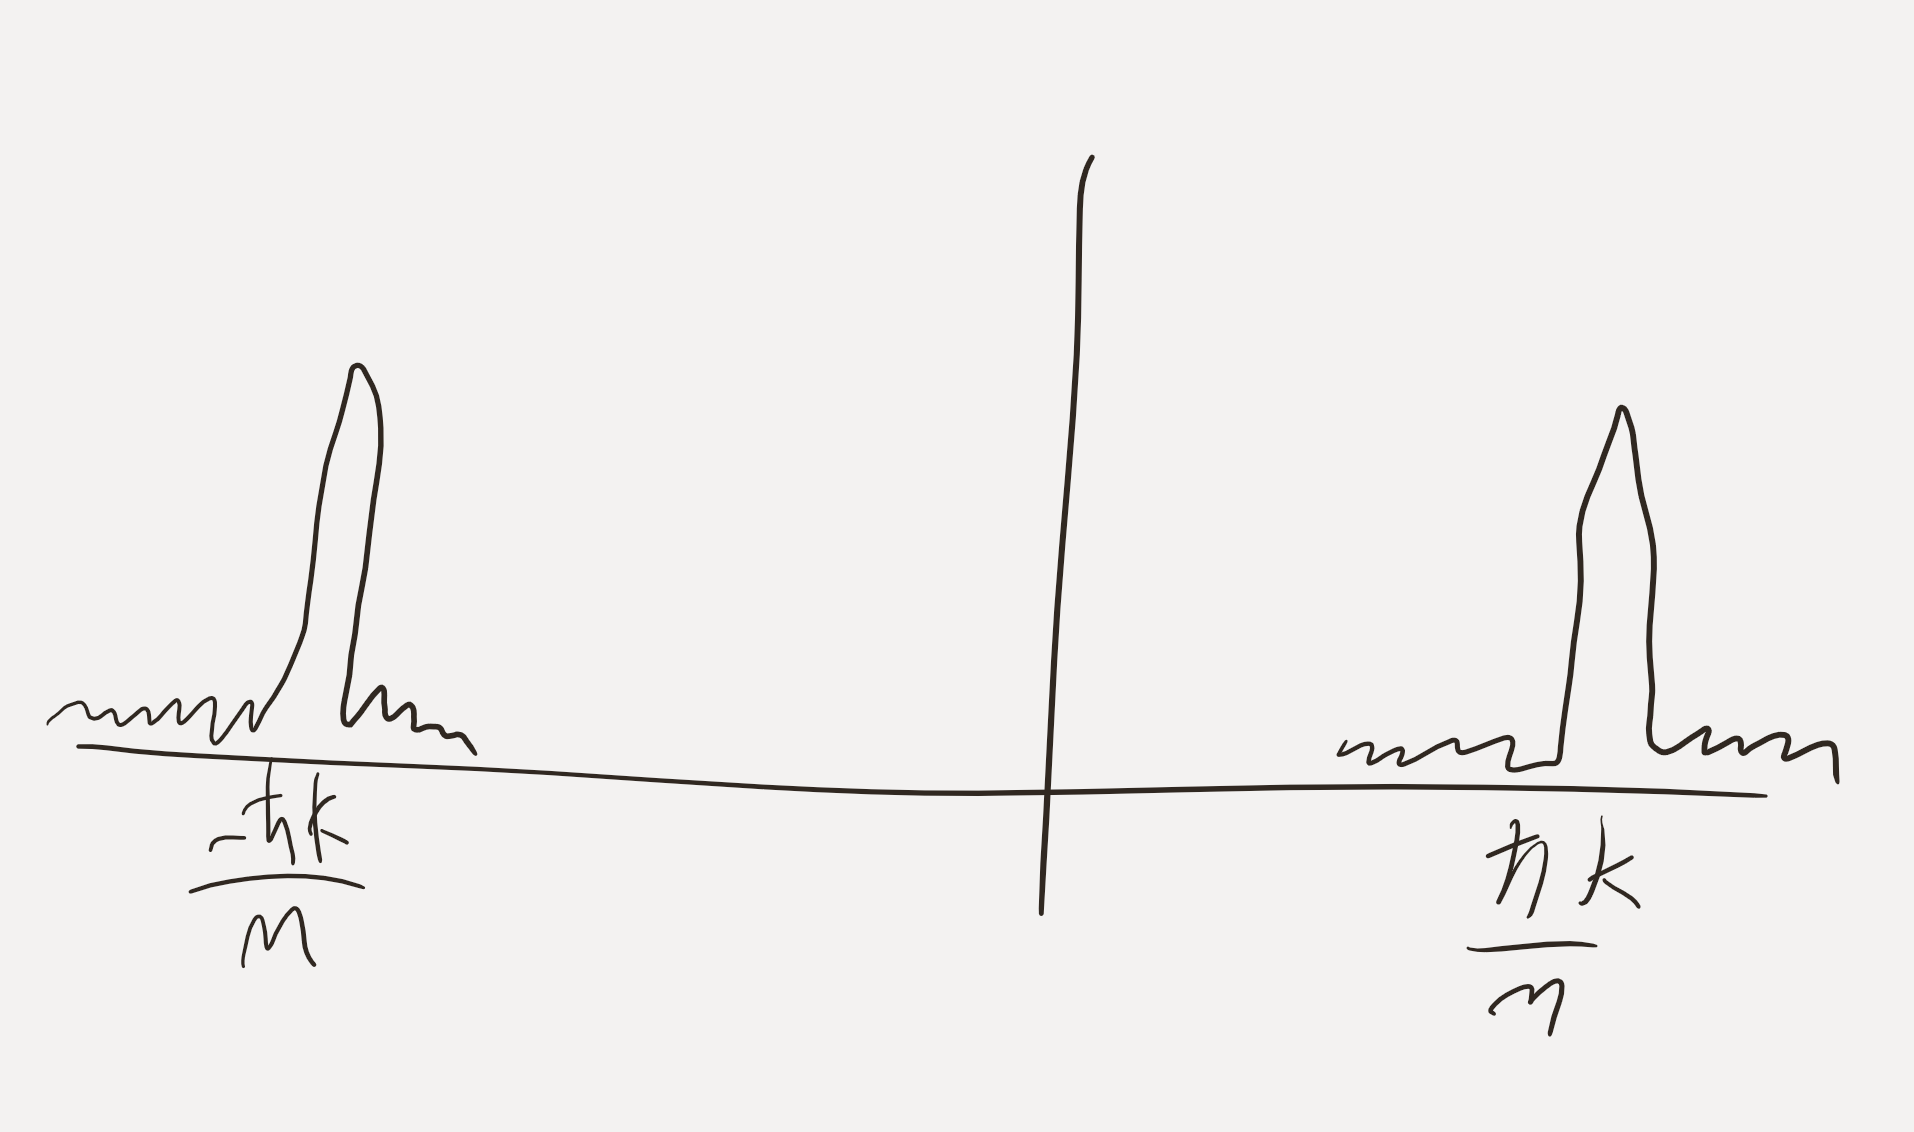
\includegraphics[width = 0.8 \textwidth]{Lecture19/1.png}

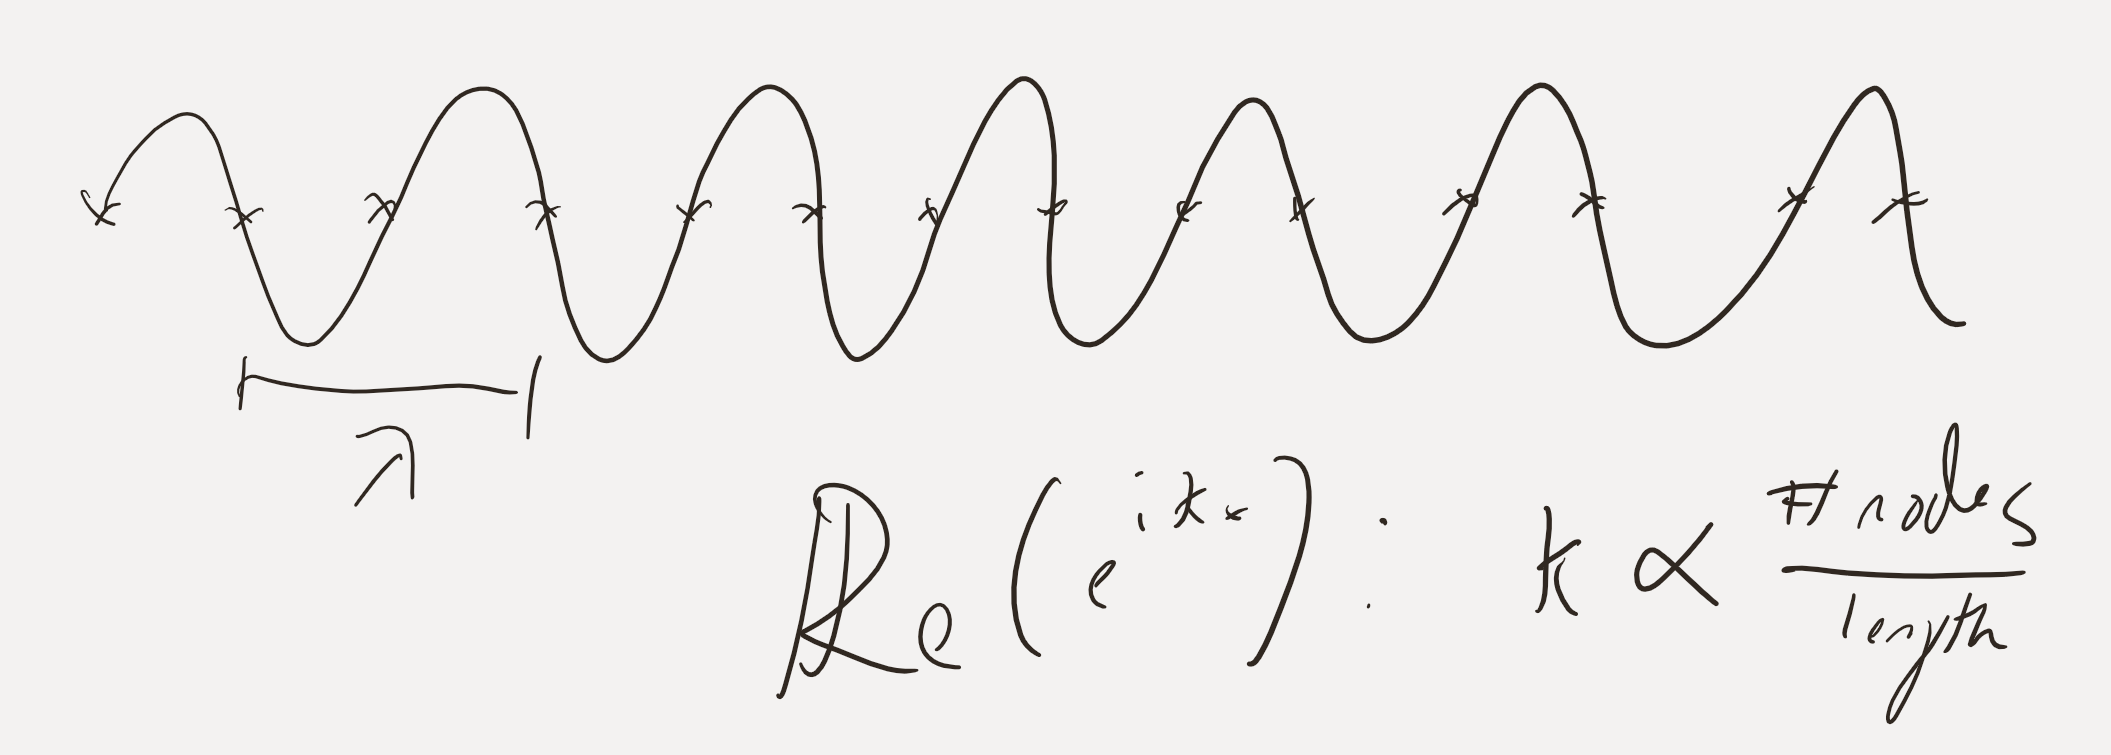
\includegraphics[width = 0.9 \textwidth]{Lecture19/2.png}

\subsection{Poll #1}

At the lowest energy state, 

$E_{n_x, n_y, n_z} = \frac{\hbar^2}{2m} \left( \frac{\pi}{a} \right)^2 (n_x^2 + n_y^2 + n_z^2) \times 3$

How many states have an energy equal to twice the lowest possible energy?

$E_{n_x, n_y, n_z} = \frac{\hbar^2}{2m} \left( \frac{\pi}{a} \right)^2 \times 6$

\subsection{Contrast with 1D}

In 1D, free particle also had degenerate eigen states $E = E_{|k|} = E_k = E_{-k}$

This can translate to symmetry of $V(x)$ = constant - Translationally symmetric potential. 

Or $V(x)$ is invariant under arbitrary translation in $x$. $V(x) = V(T_{\Delta x} x)$. $T_{\Delta x}$ is "translate by $\Delta x$". 

What about 3D cubic potential?

Degeneracy: linked to symmetry properties of $V(\vec{r})$. 

Level spacings: note while doing problem set. 

V has symmetries: if you look at a plot of V, you can’t tell which of 3 different actual directions the view might be taken from, so any solution of the TISE must also be invariant under the same change in perspective (in this case, interchange x,y or x,z or y,z.

Linear superposition of degenerate eigen states are also eigen states with same eigen energy. 

Proof: 

If $$\hat{H} \ket{\Psi_{\{n\}}} = E \ket{\Psi_{\{n\}}}$$

then $$\hat{H} \sum_{\{n\}} c_{\{n\}} \ket{\Psi_{\{n\}}} =  \sum_{\{n\}} c_{\{n\}} \hat{H} \ket{\Psi_{\{n\}}} = E \sum_{\{n\}} c_{\{n\}} \ket{\Psi_{\{n\}}} $$

They are also eigen states of the Hamiltonian operator, with the same eigen value.  More generally linear combinations of degenerate eigen states of any Hermitian operator are also eigen states with the same eigen value. 


$$\sin \left( \frac{n_x \pi x}{a} \right) \sin \left( \frac{n_y \pi y}{a} \right)$$

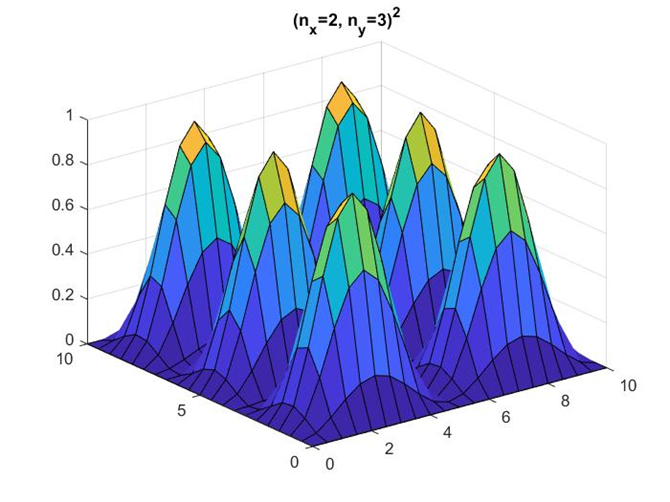
\includegraphics[width = 0.4 \textwidth]{Lecture19/3.png}
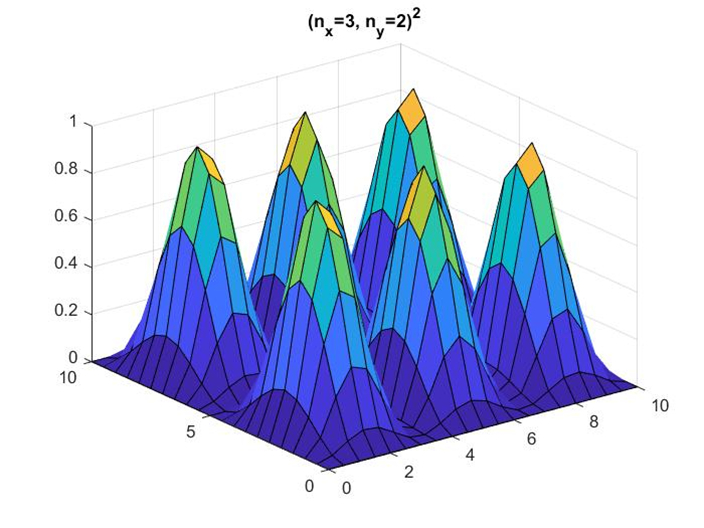
\includegraphics[width = 0.4 \textwidth]{Lecture19/4.png}

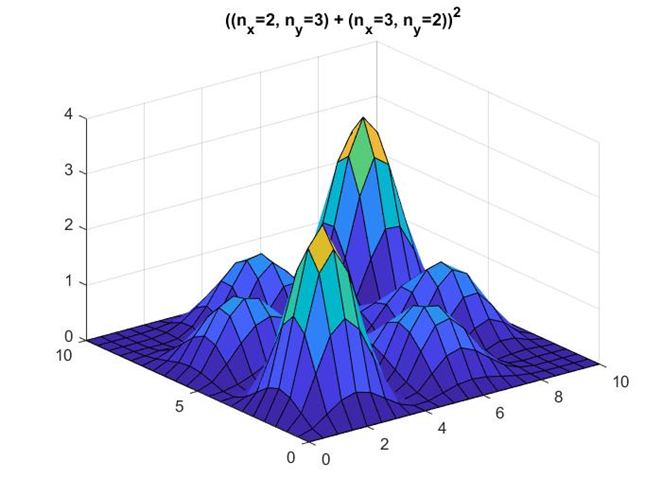
\includegraphics[width = 0.4 \textwidth]{Lecture19/5.png}
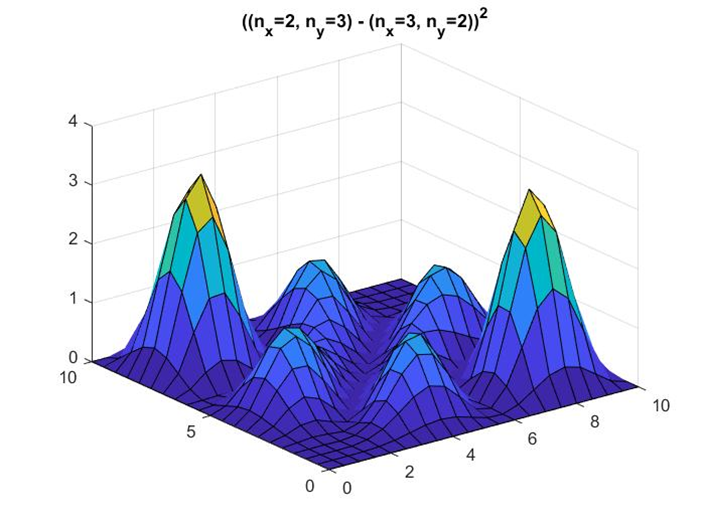
\includegraphics[width = 0.4 \textwidth]{Lecture19/6.png}

\section{Central Potentials (e.g. atoms / hydrogen)}

What comes to mind when you think about “the hydrogen atom”?

\begin{itemize}
    \item Orbitals; electron clouds, charge distribution, spdf, etc.
    \item $V ~ \frac{1}{|\vec{r}|}$
    \item Bohr radius
    \item isotopes
    \item nuclear fusion
    \item emission spectrum
\end{itemize}

This is our first example of a “real” physical system.  Within the non-relativistic limit, what terms do you think one would have to include in the Hamiltonian describing a single hydrogen atom in vacuum, in general?

What simplifying approximation(s) seem appropriate when thinking of how to define the Hamiltonian to solve in the time independent SE for “the hydrogen atom”, if you are aiming primarily to understand what colours of light would be emitted from a collection of hydrogen atoms in a fluorescent tube?

Generally have to include the kinetic energy of the proton, more generally still, should write down individual Hamiltonians for the quarks that make up the proton (kinetic energy  and interactions), and should in principle also include the Hamiltonian of the vacuum (photon bath), as the Coulomb potential is a simplification of the full EM interaction of the charged particles and the vacuum EM fields.

Assume it’s center of motion is not of interest (kinetic energy at non-relativistic speeds much less than potential energy of electron-proton binding energy.
Assume it’s internal nuclear state is “a solved problem at a few eV energy scales (shining few eV photons on the atom won’t budget the nucleus)
Assume its interaction rate with the light is very weak.



\end{document}